% generated by scripts/pkl_to_latex.py
% source PKL : tscan_v1_L8_Ne8_U5_mode-uniform_nmin2_solver-gcg_full_es_restarts10_iter300_kmax5_tol1em09_t0.05to2_N21-32c2aa6cb1ca.pkl
% scan type  : tscan
% state      : ex_singlet
% requires   : \usepackage{pgfplots} \pgfplotsset{compat=1.18}
% colours match the matplotlib PDF (tab10 cycle)
\definecolor{gmeC0}{HTML}{1F77B4}
\definecolor{gmeC1}{HTML}{FF7F0E}
\definecolor{gmeC2}{HTML}{2CA02C}
\definecolor{gmeC3}{HTML}{D62728}
\definecolor{gmeC4}{HTML}{9467BD}
\definecolor{gmeC5}{HTML}{8C564B}
\definecolor{gmeC6}{HTML}{E377C2}
\definecolor{gmeC7}{HTML}{17BECF}

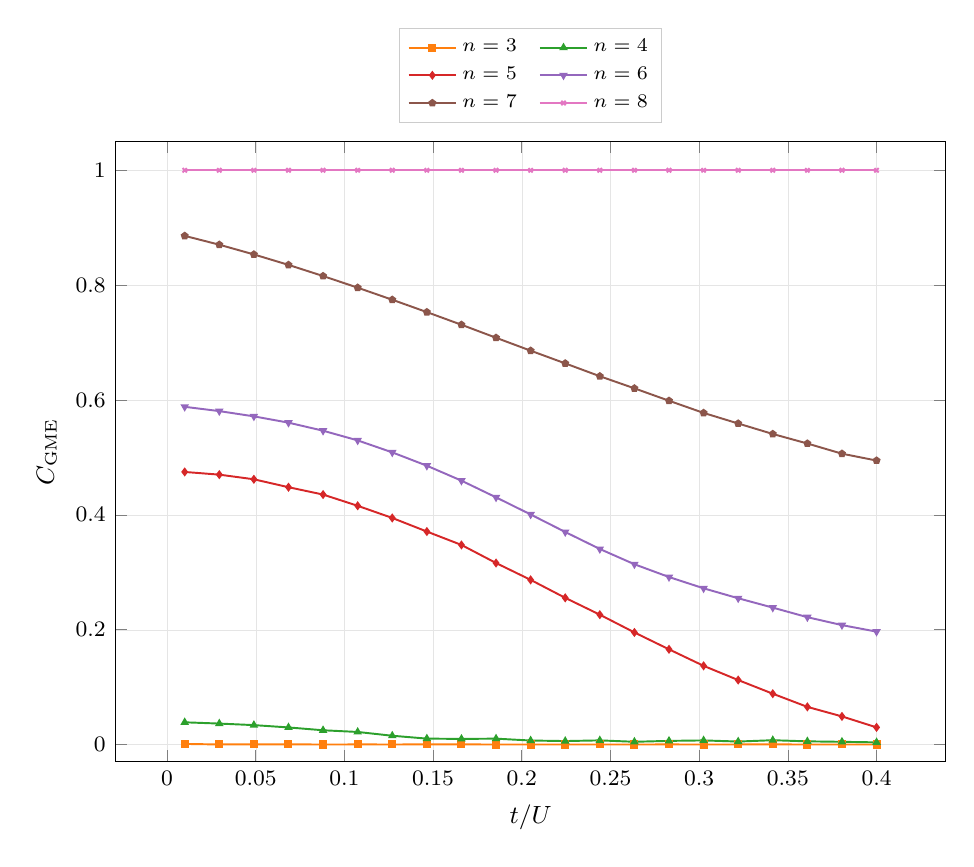
\begin{tikzpicture}
  \begin{axis}[
    width=\columnwidth,
    height=0.78\columnwidth,
    xlabel={$t/U$},
    ylabel={$C_{\mathrm{GME}}$},
    grid=both,
    grid style={line width=.1pt, draw=gray!20},
    tick label style={font=\footnotesize\rmfamily, /pgf/number format/fixed},
    label style={font=\small\rmfamily},
    scaled ticks=false,
    legend style={font=\scriptsize\rmfamily, draw=gray!40, at={(0.5,1.03)}, anchor=south, /tikz/every even column/.append style={column sep=6pt}},
    legend cell align={left},
    legend columns=2,
    ymin=-0.03,
    ymax=1.05,
  ]
    \addplot[color=gmeC1, mark=square*, mark size=1.1pt, line width=0.7pt] coordinates {
        (0.01,0.001014) (0.0295,0.000076) (0.049,0.000394) (0.0685,0.000232)
        (0.088,0.000003) (0.1075,0.000111) (0.127,0.000055) (0.1465,0.000138)
        (0.166,0.000153) (0.1855,0.000023) (0.205,0.000026) (0.2245,0.000014)
        (0.244,0.000072) (0.2635,0.000035) (0.283,0.00011) (0.3025,0.000007)
        (0.322,0.000076) (0.3415,0.000159) (0.361,0.000014) (0.3805,0.000054)
        (0.4,0.000034)
    };
    \addlegendentry{$n=3$}
    \addplot[color=gmeC2, mark=triangle*, mark size=1.1pt, line width=0.7pt] coordinates {
        (0.01,0.038681) (0.0295,0.036463) (0.049,0.033787) (0.0685,0.029741)
        (0.088,0.024807) (0.1075,0.021855) (0.127,0.015271) (0.1465,0.010277)
        (0.166,0.009755) (0.1855,0.010213) (0.205,0.006936) (0.2245,0.006019)
        (0.244,0.007183) (0.2635,0.004754) (0.283,0.00632) (0.3025,0.007125)
        (0.322,0.005181) (0.3415,0.00748) (0.361,0.005502) (0.3805,0.004687)
        (0.4,0.00376)
    };
    \addlegendentry{$n=4$}
    \addplot[color=gmeC3, mark=diamond*, mark size=1.1pt, line width=0.7pt] coordinates {
        (0.01,0.474649) (0.0295,0.469963) (0.049,0.461875) (0.0685,0.44808)
        (0.088,0.435262) (0.1075,0.415719) (0.127,0.394549) (0.1465,0.370869)
        (0.166,0.347553) (0.1855,0.316053) (0.205,0.286717) (0.2245,0.255412)
        (0.244,0.226108) (0.2635,0.195162) (0.283,0.165754) (0.3025,0.137)
        (0.322,0.112238) (0.3415,0.088474) (0.361,0.065524) (0.3805,0.048939)
        (0.4,0.029816)
    };
    \addlegendentry{$n=5$}
    \addplot[color=gmeC4, mark=triangle*, mark size=1.1pt, mark options={rotate=180}, line width=0.7pt] coordinates {
        (0.01,0.588074) (0.0295,0.580608) (0.049,0.571462) (0.0685,0.560488)
        (0.088,0.546456) (0.1075,0.529611) (0.127,0.508737) (0.1465,0.485518)
        (0.166,0.459496) (0.1855,0.430417) (0.205,0.400619) (0.2245,0.370093)
        (0.244,0.340488) (0.2635,0.313911) (0.283,0.291646) (0.3025,0.272023)
        (0.322,0.25469) (0.3415,0.238399) (0.361,0.221732) (0.3805,0.207937)
        (0.4,0.196561)
    };
    \addlegendentry{$n=6$}
    \addplot[color=gmeC5, mark=pentagon*, mark size=1.1pt, line width=0.7pt] coordinates {
        (0.01,0.885815) (0.0295,0.870385) (0.049,0.85344) (0.0685,0.835238)
        (0.088,0.815817) (0.1075,0.795543) (0.127,0.774544) (0.1465,0.753015)
        (0.166,0.730997) (0.1855,0.708321) (0.205,0.685844) (0.2245,0.663709)
        (0.244,0.641345) (0.2635,0.62025) (0.283,0.598645) (0.3025,0.577451)
        (0.322,0.559013) (0.3415,0.540781) (0.361,0.524167) (0.3805,0.50644)
        (0.4,0.494503)
    };
    \addlegendentry{$n=7$}
    \addplot[color=gmeC6, mark=x, mark size=1.1pt, line width=0.7pt] coordinates {
        (0.01,1) (0.0295,1) (0.049,1) (0.0685,1)
        (0.088,1) (0.1075,1) (0.127,1) (0.1465,1)
        (0.166,1) (0.1855,1) (0.205,1) (0.2245,1)
        (0.244,1) (0.2635,1) (0.283,1) (0.3025,1)
        (0.322,1) (0.3415,1) (0.361,1) (0.3805,1)
        (0.4,1)
    };
    \addlegendentry{$n=8$}
  \end{axis}
\end{tikzpicture}
